\section{Experimental Evaluation}
\label{sec:evaluation}

In this section we are going to present the results gotten from our experimental evaluation.

\sd{quando hai definito i paragrafi linkali}


In order to get the reader accustomed with what we are evaluating, we present only a subset of the whole family of instances that we have evaluated for this project. We specifically center our focus towards a 9x9 instance, so that the reader can understand how different solutions compare given the same problem to solve. In case you are more interested, you can find more plots in our drive \sd{drive link!}.


\subsection{Can we evaluate difficulty of a Futoshiki before solving it?}
\label{subsec:futoshiki_difficulty}
It is important to stop for a moment and assess a crucial factor: as we have already explained in \Cref{subsec:backtrack} how Futoshiki has dynamic placed constraints, which in turn implies that the assumption we can make on the input are less strict w.r.t. Sudoku. This means that by receiving as input only the number of constraints, without knowing whey they are placed and how they are intertwined one to another, it is extremely hard to define the actual "difficulty" of the problem. It is easy to see that with a simple manipulation of the constraints presented in \Cref{fig:futoshiki_example}, one could not have easily understood the chain between values 1-4. Another factor to take into account is where the initial numbers are placed and how many we have. It is true as the number of constraints that we have increases, the more variables we can fix and therefore the less big the search spaces becomes, but if those constraints are placed in a "bad way", one could not find the solution easily.

We can also say that the "size matters" in this case it not strictly true. One could imagine a puzzle of a specific size and one of a slightly bigger size: let's say 9x9 and 10x10. Given those as inputs, as the correlation among constraint is so important that just like for the amount of numbers placed, they might not lead to an "easier" or "harder" puzzle by default.
To wrap up this consideration, we can safely say that if we are only given number of constraints, number of initialized cells and size of the problem it is not possible to give a precise estimate over a metric to evaluate the "difficulty" of the problem.

\subsection{Experimental Setup}
We now move onto some first consideration on the underlying Hardware, to have an idea of what the numbers that we are going to see actuallyh mean.

All experiments were conducted on a high-performance computing cluster with the following specifications:
\begin{itemize}
    \item \textbf{Hardware:} 126 nodes with Intel Xeon processors.
    \item \textbf{Network:} 10Gb/s Ethernet with Infiniband/Omnipath options.
    \item \textbf{Software:} Linux CentOS 7, GCC 9.1, MPICH 3.2.
    \item \textbf{Test Cases:} Various puzzles from 5×5 to 11×11, including "hard" instances.
\end{itemize}

\subsection{Impact of Pre-coloring Optimization}
\label{subsec:precoloring_performance}
As we have already discussed in \Cref{subsubsec:precoloring}, the precoloring procedure helps us at doing some pre computation, which in turn lets us reduce the search space of our solution. In \Cref{fig:precoloring_improvement} we see how by performing precoloring gives us better results w.r.t. the standard brute force approach. In the X axis we have 3 different 9x9 problems to be solved, and in the Y axis the total time measured in seconds for \textit{the solving time of our algorithm only}.

\begin{figure}[htbp]
\centering
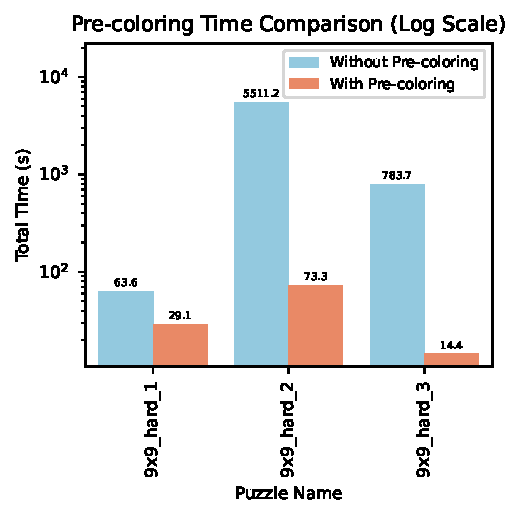
\includegraphics[width=0.9\linewidth]{imgs/precoloring_comparison.pdf}
\caption{Comparison of execution times for some 9x9 futoshiki problems}
\label{fig:precoloring_improvement}
\end{figure}


This figure lets us understand that by employing this technique we can see up to 54x speedup, like in the case of the instance \textit{9x9\_hard\_3}. This means that even if we have a little bit of overhead to apply the list coloring solution, we can still see great improvements over the baseline. For this reason we chose to employ precoloring on all of the following case studies, so that we both reduce the amount of variables in our comparison while introducing several fold speedup in our proposed solution.

\subsection{What the factor are we talking about?}
We have already mentioned that our solutions have a parameter presented as \textit{Configurable Factor}. We said that this factor lets us tweak the ratio between the jobs being scheduled and the underlying computational unit(either a thread for the OpenMP case, or a CPU for the MPI one). From an high level point of view we can think it as a knob that lets us choose at our will the amount of "pressure" that we are putting the underlying system in.

From a more formal point of view, given a factor F and the number of underlying computational units C, our preprocessing algorithm aims at going deeper and deeper into the search space by exploring the backtrack tree until it does not find an amount of puzzles to solve P such that:
\[
    F * C \leq P
\]

This lets us play around to find the best possible ratio, which therefore lets us find the maximum amount of "stress" to put our computational units at before we have generated too many jobs for them.

In fact, we have run several tests to assess which factor could be the best one to choose from, so we now present our \textit{Factor Analysis} that we have devised to pick it.


\begin{figure}[htbp]
\centering
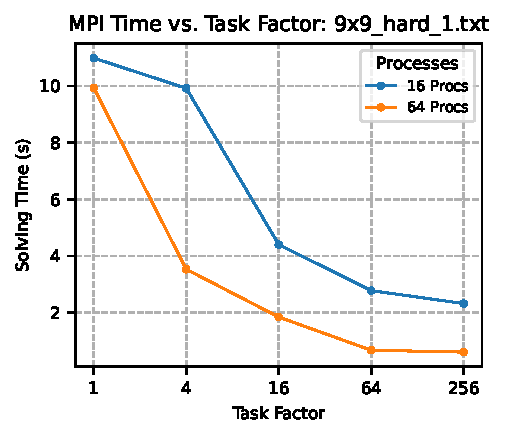
\includegraphics[width=0.9\linewidth]{imgs/factor_analysis_mpi_9x9_hard_1.pdf}
\caption{factor analysis for MPI}
\label{fig:factor_analysis_mpi}
\end{figure}

\begin{figure}[htbp]
\centering
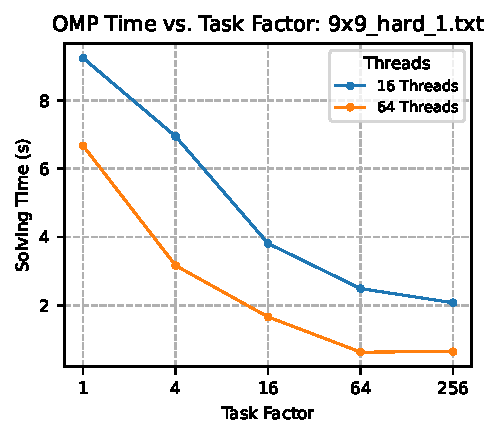
\includegraphics[width=0.9\linewidth]{imgs/factor_analysis_omp_9x9_hard_1.pdf}
\caption{factor analysis for OMP}
\label{fig:factor_analysis_omp}
\end{figure}

\begin{figure}[htbp]
\centering
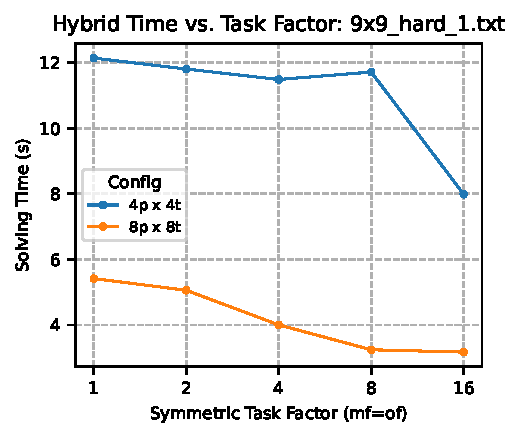
\includegraphics[width=0.9\linewidth]{imgs/factor_analysis_hybrid_9x9_hard_1.pdf}
\caption{factor analysis for hybrid solution}
\label{fig:factor_analysis_hybrid}
\end{figure}

From \Cref{fig:factor_analysis_mpi} and \Cref{fig:factor_analysis_omp} we can see that we have a good slope in the decreasing of the solving time of our solution with 16 processors/threads up until 64, and then we start to stabilize. In order to keep things simple, we have opted for this value.

As for the hybrid, we have faced the issue on "how can we evaluate MPI and OMP solutions"? In order to provide some interesting results, we have decided to abstract away from the actual implementation of the worker (MPI or OMP), and we have therefore decided to treat a processor in MPI as the same as the threads for OMP. This modeling simplification is going to help us in \Cref{subsec:hybrid_results} when evaluating how the hybrid solution works under several different configurations.
\sd{check if this link works after doing hybrid results}

After having taken this necessary detour, we can move towards finding the best factor for the hybrid one: we can see from \Cref{fig:factor_analysis_hybrid} that if we consider the symmetric factor 8, which means setting Mpi Factor to 8 and Openmp Factor to 8, if we take this approximation into account (considering processors = threads), we can see how 8*8=64 is also a fairly good factor in this case.


For this reason, we have decided to set for the following runs MPI and OMP factor to 64, and for the hybrid the MPI Factor to 8 and its symmetric counterpart to 8, so that we would have a factor of 64 "computational units" across the board.


\subsection{Parallel Performance Analysis}

After having understood how hard it is to evaluate the difficulty of our problem \textit{a priori}, and having set the ground for our base configuration (hardware used, pre coloring algorithm, factor selected), we can finally move into the evaluation of how our parallel solutions work.

\subsubsection{Solving times for MPI and OMP}
\label{subsubsec:solving_times_mpi_omp}

We start off by showing how our MPI and OMP solutions work with a 9x9\_hard instance and a 10x10\_hard instance (note that the "hard" concept comes from how the website from which we have taken the problems from ranked them. Here are the 2 main sources from which we downloaded \cite{puzzle_futoshiki,puddelbee} and converted images to compatible representation via a custom parser which we have devised in order to gather data).

Please note that as the cluster has a maximum amount of thread per node set to 64, we cannot gather data in the case of 128 threads due to HW constraints. This is the main reason why in the following plots there is not going to be an entry for OMP with 128 Computational units.


We start off by showing a 9x9 instance in \Cref{fig:comparison_solving_time_9x9}. On the x axis we have the number of computational units that we are using, and on the Y axis the time it required for our algorithms to find a valid permutation of numbers to solve the puzzle.

We can see that, as we expect, as the number of computational units increase, the solving time for our problem decreases as we can extract more and more parallel work.

The red dotted line serves as a baseline, as it is the time required for our sequential algorithm to find a solution and it is going to be present in the next graphs also, so that one can easily understand how a given parallel implementation compares w.r.t. the sequential one.

We can see that for 1 and 2 we have values which are in the range of the sequential algorithm minus some seconds of delta in the measurement and this is because, as we have already presented in the \Cref{sec:solution} we have decided to opt for the sequential algorithm to remove the overhead given by OMP and MPI.
\sd{occhio}

\begin{figure}[htbp]
\centering
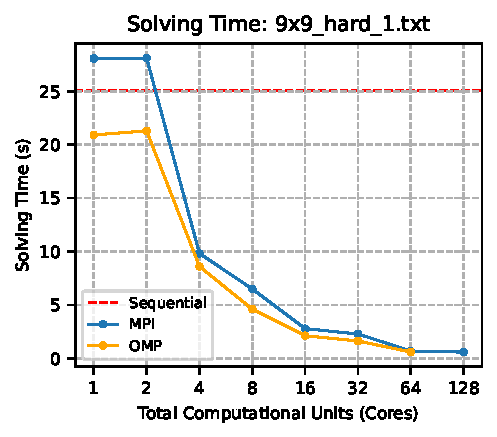
\includegraphics[width=0.9\linewidth]{imgs/comparison_solving_time_9x9_hard_1.pdf}
\caption{Solving time comparison for a 9x9 instance}
\label{fig:comparison_solving_time_9x9}
\end{figure}

We now move towards a 10x10 instance. In \Cref{fig:comparison_solving_time_10x10} we see something strange: every parallel implementation is consistently worse w.r.t. solving time compared to the sequential solution (minus some cases like the 4,8 and 16 CU which have little to no actual increase in performance). 

This is very interesting, because by looking at the absolute value of the solving time we can note that even the sequential algorithm is taking less than 0.01 second to find the solution. This lets us draw two necessary conclusions:
\begin{enumerate}
    \item As we have stated in \Cref{subsec:futoshiki_difficulty}, the size alone is not a factor which directly implies the difficulty of the problem. We can see that the absolute time to solve the 9x9 and 10x10 are vastly different, even if someone might at a first glance say "if we have more cells we should have higher execution times". This does not always hold if we do not consider all of the aforementioned variables.
    \item Parallel solutions introduce some overhead, either the message passing infrastructure needed for the MPI framework to process messages, or the locks needed to achieve high efficiency shared memory reading and writing when accessing critical parts of code. Such overhead is usually mitigated by the fact that the overall performance increase in finding a solution is higher than the overhead introduced by parallelizing the work. This is not the case for these specific families of problems: as the sequential solution is already extremely fast, it does not make sense to parallelize it, and therefore we can conclude that this family of instances are not tailored or our parallel solution analysis.
\end{enumerate}

For such reasons, we are going to move to analyze only the family of 9x9 instances, as they are more interesting and actually give us some interesting data and points to reason about w.r.t. just saying "for the 10x10 instance we have a degradation in performance".

\begin{figure}[htbp]
\centering
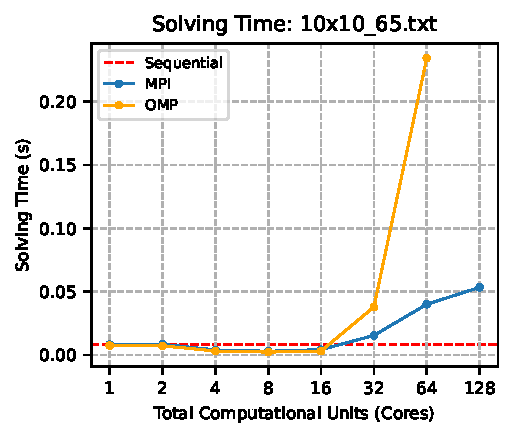
\includegraphics[width=0.9\linewidth]{imgs/comparison_solving_time_10x10_65.pdf}
\caption{Solving time comparison for a 10x10 instance}
\label{fig:comparison_solving_time_10x10}
\end{figure}

\subsubsection{How well does parallel solution perform compared to sequential?}
\label{subsubsec:speedup_efficiency}

Now that the reader has understood how configurations and difficulty of the puzzles impact the overall execution time, he might ask himself "is there a metric to evaluate how much better the parallel solutions are compared to the sequential one?"

Turns out that we have such metrics. We know that if we have a task and we parallelize it, we can use the \textit{Speedup} concept to understand how much better it gets, and it is presented as:
\[
S = \frac{Execution\_time\_sequential}{Execution\_time\_parallel}
\]
This means that the lower the execution time is when parallelized, the higher the speedup is going to be. In \Cref{fig:speedup_9x9} we show the speedup that we can reach with our solution. On the x axis w.h. the computational units, whereas in the Y axis we have the speedup value. The red line represents the theoretical speedup that we can reach, so assuming that the parallelization of the task introduces absolutely 0 overhead.

An interesting takeaway from this plot is that while we reach a speedup which is close to the ideal one in the 0-20 computational units case, we can see how by increasing the number of units we have a speedup value which does not grow as fast as the theoretical one. From this we can conclude that:
\begin{enumerate}
    \item As the number of computational units increase, we introduce higher overhead due to the message passing or the shared variables accesses, which is not much if we have "few" computational units, but as the number goes up the overhead is getting a little bit bigger, therefore impacting the overall speedup.
    \item The fact that the speedup does not grow as fast as the ideal one does not mean that the solution gets slower: It is still faster than the sequential solution.
\end{enumerate}


\begin{figure}[htbp]
\centering
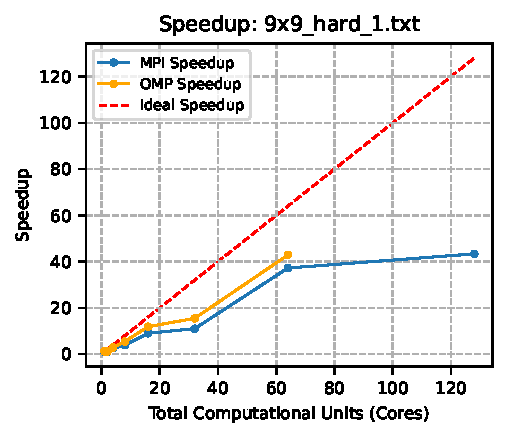
\includegraphics[width=0.9\linewidth]{imgs/comparison_speedup_9x9_hard_1.pdf}
\caption{Speedup of parallel solutions}
\label{fig:speedup_9x9}
\end{figure}

We can now move into the second metric that we can use to evaluate our parallel algorithm w.r.t. the sequential one: the \textit{Efficiency}. This is a derivative parameter which is dependent on the speedup, and it can be expressed as:
\[
E = \frac{Speedup}{\# computational\_units}
\]

This parameter is basically relating the speedup(how well the parallel solution is w.r.t. the sequential one) with the number of units available. This parameter is therefore going to tell us how well the available cores are being used.

\Cref{fig:efficiency_9x9} we can see how efficiency is evaluated in our solutions. We see how the overall efficiency decreases as the number of computational units increase. This is expected: efficiency is a mirror of the speedup, so as we have noticed how that was decreasing due to the overhead of the underlying technologies used, we should expect that the amount of work to be done is going to decrease as the amount of available computational cores increases. We can however note that 
\begin{enumerate}
    \item OMP is strictly dominating the MPI efficiency plot, and this tells us that OMP overhead due to the shared memory access is stricly lower than the message passing approach used by MPI, which is fairly interesting. 
    \item We have a high decrease in efficiency when increasing the number of cores from 1 to 2,4 but then we stabilize as the number of core increases. This is expected as, since the efficiency explains how much each core is contributing and "kept busy" to achieve the final goal, as we increase the amount of available cores we give less amount of work to every core which is expected.
\end{enumerate}
\sd{we can say in future works play with factor to see how to maximize efficiency of solution which is good!}

\begin{figure}[htbp]
\centering
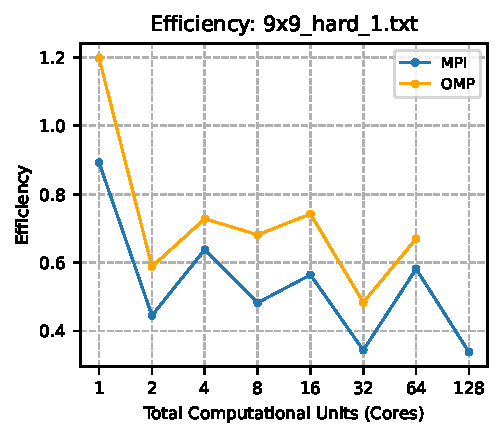
\includegraphics[width=0.9\linewidth]{imgs/comparison_efficiency_9x9_hard_1.pdf}
\caption{Efficiency of parallel solutions}
\label{fig:efficiency_9x9}
\end{figure}




\subsubsection{MPI Scalability}
Table \ref{tab:mpi_scaling} presents MPI performance across multiple nodes:

\begin{table}[htbp]
\caption{MPI Strong Scaling (9×9 Hard Puzzle)}
\begin{center}
\begin{tabular}{@{}ccccc@{}}
\toprule
\textbf{Processes} & \textbf{Time (s)} & \textbf{Speedup} & \textbf{Efficiency} \\
\midrule
1 & 35.84 & 1.00 & 100.0\% \\
2 & 18.21 & 1.97 & 98.5\% \\
4 & 9.45 & 3.79 & 94.8\% \\
8 & 5.11 & 7.01 & 87.6\% \\
16 & 3.02 & 11.87 & 74.2\% \\
32 & 2.25 & 15.93 & 49.8\% \\
64 & 2.05 & 17.48 & 27.3\% \\
128 & 2.01 & 17.83 & 13.9\% \\
\bottomrule
\end{tabular}
\end{center}
\label{tab:mpi_scaling}
\end{table}

MPI maintains higher efficiency than OpenMP at moderate scales due to better memory locality, but communication overhead becomes significant beyond 32 processes.

\subsubsection{OpenMP Scalability}
Table \ref{tab:openmp_scaling} shows OpenMP performance with increasing thread counts on a single node:

\begin{table}[htbp]
\caption{OpenMP Strong Scaling (9×9 Hard Puzzle)}
\begin{center}
\begin{tabular}{@{}ccccc@{}}
\toprule
\textbf{Threads} & \textbf{Time (s)} & \textbf{Speedup} & \textbf{Efficiency} \\
\midrule
1 & 35.84 & 1.00 & 100.0\% \\
2 & 18.45 & 1.94 & 97.2\% \\
4 & 9.78 & 3.67 & 91.7\% \\
8 & 5.42 & 6.61 & 82.6\% \\
16 & 3.18 & 11.27 & 70.4\% \\
32 & 2.36 & 15.19 & 47.5\% \\
64 & 2.35 & 15.25 & 23.8\% \\
\bottomrule
\end{tabular}
\end{center}
\label{tab:openmp_scaling}
\end{table}

OpenMP shows excellent efficiency up to 8 threads, with diminishing returns beyond 16 threads due to NUMA effects and increased synchronization overhead.


\subsubsection{Hybrid Performance}
The hybrid solver demonstrates superior scalability by combining both paradigms:

\begin{table}[htbp]
\caption{Hybrid Scaling with Various Configurations (11×11 Hard Puzzle)}
\begin{center}
\begin{tabular}{@{}cccccc@{}}
\toprule
\textbf{MPI} & \textbf{OMP} & \textbf{Total} & \textbf{Time} & \textbf{Speedup} \\
\textbf{Procs} & \textbf{Threads} & \textbf{Cores} & \textbf{(s)} & \\
\midrule
1 & 1 & 1 & 142.36 & 1.00 \\
1 & 4 & 4 & 37.82 & 3.76 \\
2 & 2 & 4 & 36.94 & 3.85 \\
4 & 1 & 4 & 38.45 & 3.70 \\
2 & 8 & 16 & 10.28 & 13.85 \\
4 & 4 & 16 & 9.87 & 14.42 \\
8 & 2 & 16 & 10.95 & 13.00 \\
4 & 16 & 64 & 5.12 & 27.80 \\
8 & 8 & 64 & 5.03 & 28.31 \\
16 & 4 & 64 & 5.38 & 26.46 \\
\bottomrule
\end{tabular}
\end{center}
\label{tab:hybrid_scaling}
\end{table}

The hybrid approach achieves the best overall speedup (28.3×) by effectively utilizing both parallelization levels. The 8×8 configuration (8 MPI processes with 8 OpenMP threads each) provides optimal performance for 64 cores.

\subsection{Task Generation Factor Analysis}
We investigated the impact of the task generation factor—a multiplier that controls work unit granularity. Figure \ref{fig:task_factor} shows performance variation with different factors:

\begin{figure}[htbp]
\centering
\includegraphics[width=0.9\linewidth]{images/precoloring }
\caption{Performance impact of task generation factor for 64 cores. Optimal performance occurs around factor = 4-8.}
\label{fig:task_factor}
\end{figure}

Optimal performance occurs around factor = 4-8, balancing sufficient parallelism against overhead. Lower factors cause load imbalance, while higher factors increase coordination overhead.

\subsection{Weak Scaling Analysis}
To evaluate scalability with increasing problem size, we conducted weak scaling experiments where puzzle size grows proportionally with processor count:

\begin{table}[htbp]
\caption{Weak Scaling Efficiency}
\begin{center}
\begin{tabular}{@{}ccccc@{}}
\toprule
\textbf{Cores} & \textbf{Puzzle} & \textbf{Time (s)} & \textbf{Efficiency} \\
\midrule
1 & 5×5 & 0.23 & 100.0\% \\
4 & 7×7 & 0.31 & 92.7\% \\
16 & 9×9 & 0.45 & 87.3\% \\
64 & 11×11 & 0.68 & 79.4\% \\
\bottomrule
\end{tabular}
\end{center}
\label{tab:weak_scaling}
\end{table}

The solver maintains good weak scaling efficiency, demonstrating its ability to handle larger problems with proportionally more resources.

\subsection{Performance Summary}
Figure \ref{fig:speedup_comparison} summarizes the speedup achieved by each implementation:

\begin{figure}[htbp]
\centering
\includegraphics[width=0.9\linewidth]{images/speedup_chart.png}
\caption{Speedup comparison across all implementations. The hybrid approach consistently outperforms single-paradigm solutions.}
\label{fig:speedup_comparison}
\end{figure}

Key observations:
\begin{itemize}
    \item \textbf{Sequential Optimization:} Pre-coloring provides 14× speedup, essential for all parallel versions
    \item \textbf{Shared Memory:} OpenMP excels within a single node but plateaus at 32 threads
    \item \textbf{Distributed Memory:} MPI scales better across nodes but has higher communication overhead
    \item \textbf{Hybrid Approach:} Combines strengths of both paradigms, achieving best overall performance
\end{itemize}